\documentclass[fleqn]{article}

\usepackage{graphicx, fullpage, amssymb, amsmath}
\usepackage{placeins}

\begin{document}

\centerline{\sc \large EECS 405 - Project Report}
\vspace{.5pc}
\centerline{\sc Nathan McKinley (ndm25) and Umang Banugaria (uxb3)}
\centerline{\it April 22, 2013}
\vspace{2pc}

\section{Abstract}
We sought to examine the properties of B-trees and B+-trees under the no-coalescing model which is usually chosen in industry.  We found that under some insert/delete workloads for uniformly random key selection, the no-coalescing model performs better in time.  In all cases, the no-coalescing model performs worse in space: its use of the allocated space sometimes drops below the 50\% minimum which is enforced when coalescing is on.

We also found that the tree height is greater when coalescing is turned on; although we did not test time for queries in out experiments, this indicates that performing sufficiently many queries will cause coalescing to be preferable.

\section{Introduction}
B+-tree-based indices are often used in database systems in order to improve query time.  Maintaining these indices is a time cost which is balanced by the benefit of having a smaller tree and using the space which you have allocated more efficiently.  Some database systems used in industry choose to turn off this maintenance, or to perform it only occasionally when the database is under very light load.  When the maintenance is turned off, the B-tree is not required to maintain its constraint that all nodes be at least 50\% full.  The index will split nodes as usual when they become overfull, but never merge them back together, instead deleting them when they become completely empty.  Noticing an underflow will not cause a merge-and-split or even a merge.

We wanted to test what conditions would lead to this being a beneficial choice, so we implemented a B-tree and B+-tree in python with a convenient command-line interface.  We implemented these trees capable of taking in key size, data record size, index pointer size, data pointer size, and block size.  These trees also take in a boolean parameter for whether or not they should coalesce when they detect an underflow.  See section 3 for the implementation details.

We also implemented a visualizer GUI which allows control over the simulation.  See section 4 for the implementation details of the visualizer.

\section{Tree Implementation}

For this project, we chose to implement two different tree structures: B trees and B+ trees.  Both tree structures are a dense index and reside in main memory.  They can each take in various parameters to allow for different order trees.  They also provide a set of functions to perform operations on the tree and gain information about the tree.  Since the purpose of this project is to explore the change in performance as the various parameters of the trees are modified, the customizable parameters are essential.  The parameters that can be set when creating a tree are:

\begin{enumerate}
\item
the key size
\item
the size of a data record
\item
the size of a data record pointer
\item
the size of a block pointer
\item
the block size
\item
whether the trees will perform coalescing when underflows occur.
\end{enumerate}
Once the trees are created, the following three operations that can be performed on the trees are:
\begin{enumerate}
\item
insert(key):  inserts the key into the tree index
\item
delete(key): deletes the key from the tree index if it is in the index.  if the key is not in the index, nothing will be done
\item
lookup(key): returns the level of the tree where there is a data pointer with a matching key.  The the case of B+ trees, this will always be the height of the tree but in B trees, it can be anywhere between 1(root) and the height.  If the key does not exist in the tree, -1 is returned
\end{enumerate}

To learn more about the structure of the tree that is created after insertions and deletions, various functions provided by both tree implementations can be used.  The following five functions are available:
\begin{enumerate}
\item
height():  returns the height of the tree
\item
numIndexBlocks(): returns the number of internal and leaf nodes being used within the tree index
\item
numDataBlocks(): returns the minimum number of blocks that would be needed to store all of the data.  this is based on the block size and data record size
\item
numElements(): returns the number of data record pointers stored in the tree
\item
storageUtil(): returns the fraction of the space used in the internal and leaf blocks.  this is computed by taking the space required by the keys, data record pointers, and block pointers and dividing it by the total space allocated to the blocks for the internal and leaf nodes.
\end{enumerate}
Since these trees were implemented to be part of a simulation, they do not actually store any data records, only the keys are stored.  To determine when a split or merge is needed, we compute the order of internal and leaf nodes based on the parameters that were set when the tree was created.  This allows us to vary the parameters to form different order trees independently of how the pointer and key data is stored in memory.

\section{GUI}

The GUI was implemented in TKinter, the standard python GUI library.  It has three menus available.  The first is for control of the window, which allows printing to postscript (the best way to view trees with gigantic branching factors), and exiting.  The second is for control of the display, which allows resizing of the text in the window.  The third is for control of the simulation, and allows for entering of new parameters to the simulation, as well as re-running the simulation.\\

The GUI is inherited primarily from the NLTK toolkit's TKinter tree-drawing method.  We convert our B-plus trees into NLTK-style trees, where each node represents a B-tree node and has as its children, in order, the children of the B-plus tree.  Then, we tell the NLTK-drawing toolkit to draw the tree in the canvas which is in the center of the GUI.

Included here are screenshots of the GUI in all modes of operation:

\begin{figure}[h!]
\centerline{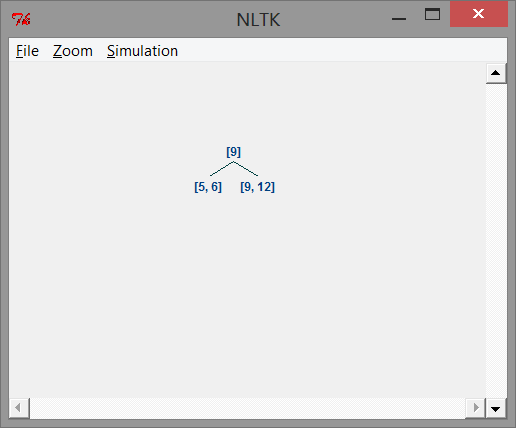
\includegraphics{Images/gui1.png}}
\caption{The GUI in its standard form, holding a very small B+ tree}
\end{figure}

\begin{figure}[h!]
\centerline{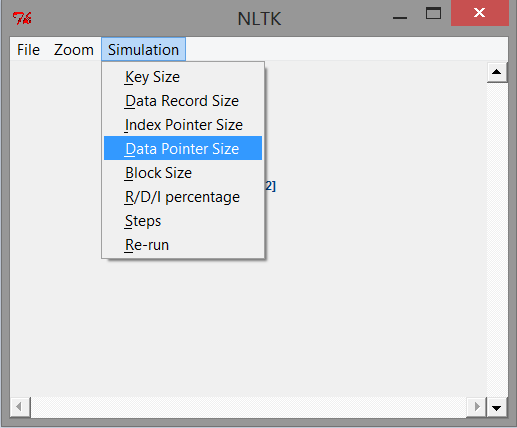
\includegraphics{Images/gui2.png}}
\caption{The simulation menu, allowing for adjustments to the simulation parameters}
\end{figure}

\begin{figure}[h!]
\centerline{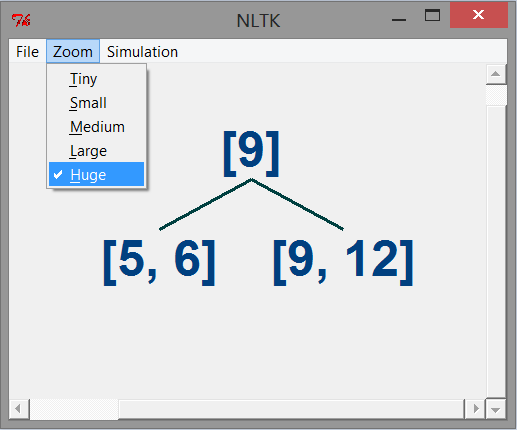
\includegraphics{Images/gui4.png}}
\caption{The menu allowing for modification to the size of the tree, inherited from NLTK}
\end{figure}

\begin{figure}[h!]
\centerline{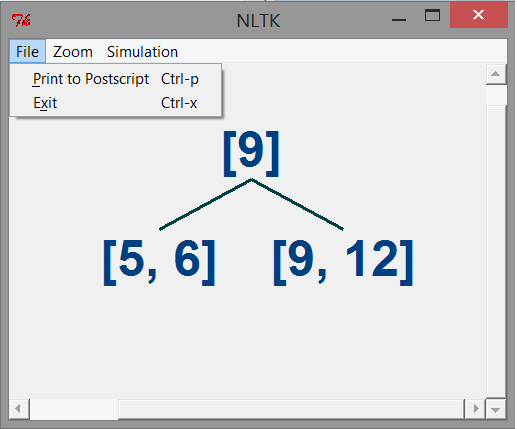
\includegraphics{Images/gui3.png}}
\caption{The menu allowing for easier display in postscript, inherited from NLTK}
\end{figure}

\begin{figure}[h!]
\centerline{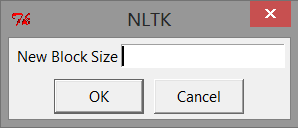
\includegraphics{Images/gui5.png}}
\caption{The GUI for inserting new parameters; in this case, block size.}
\end{figure}

\begin{figure}[h!]
\centerline{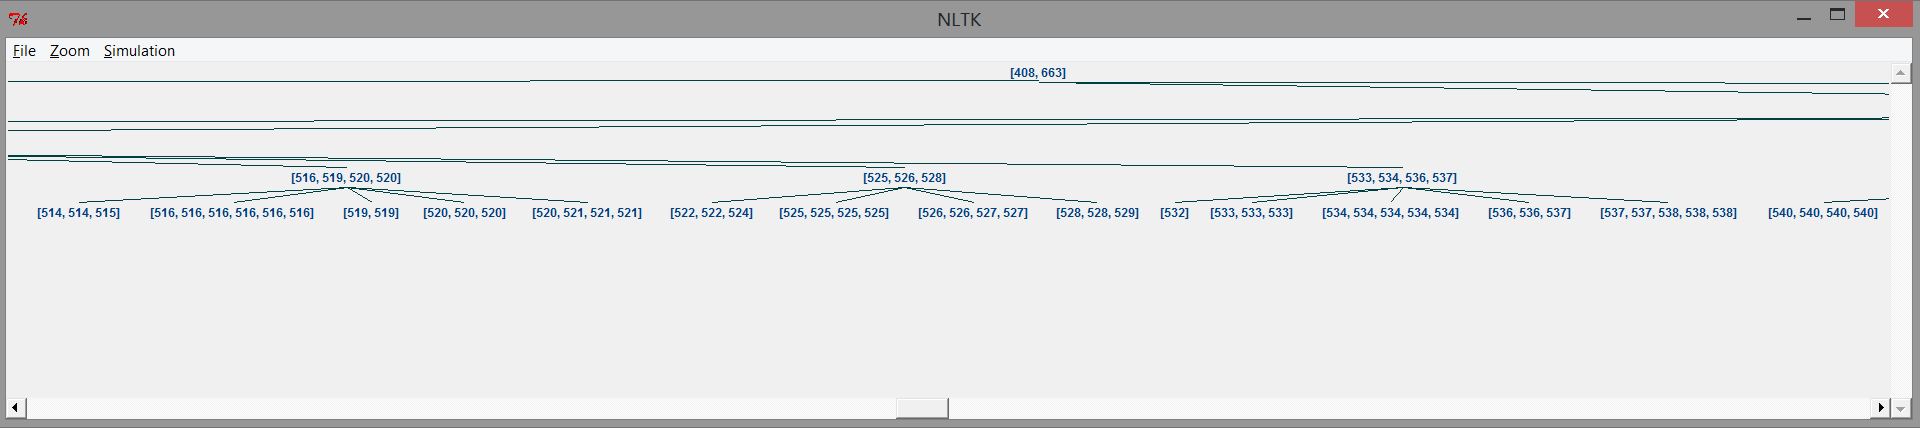
\includegraphics[width=1.2\linewidth]{Images/gui7.png}}
\caption{The GUI in its standard form, holding a very large B+ tree, uncoalesced.  We can see underfull nodes here, like the one third from the left.  This displays a potential problem of the GUI; very very large trees have a branching factor far too high to be easily seen all at once}
\end{figure}

\begin{figure}[h!]
\centerline{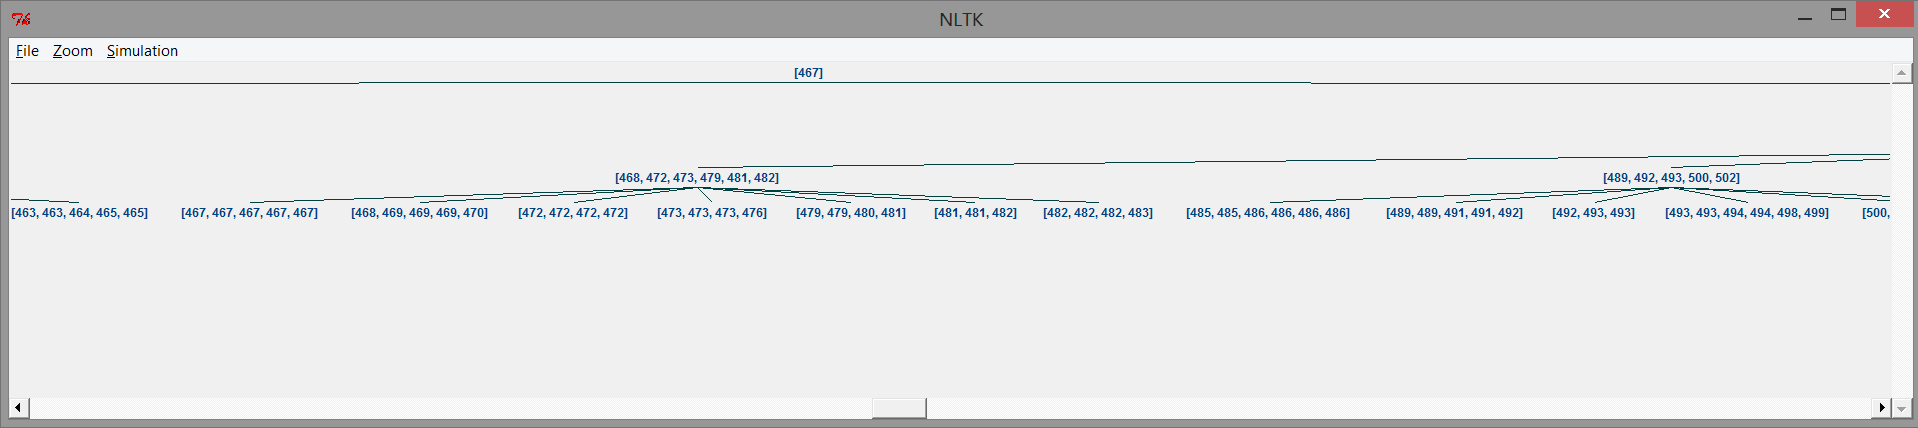
\includegraphics[width=1.2\linewidth]{Images/gui8.png}}
\caption{The GUI in its standard form, holding a very large B+ tree, coalesced.  We can see no underfull nodes here.  Additionally, we can see that there is only one root node, instead of two as in figure 6; this is because we have fewer blocks overall.}
\end{figure}

\clearpage

\section{Simulation}
The simulation class takes in all the arguments of the tree class, as stated above in section 3.  It also takes in parameters for type of tree to simulate, and insert-load, delete-load, and search-load, which should be percentages which add to 1.0, and a number of steps to run.  The simulation has an execute\_insert, execute\_delete, and execute\_read method, each of which take in a key, and will modify the tree appropriately, so it can be used as an interface to the output B+-tree or B-tree.\\

As its core method, the simulation class has a run() method.  This method initializes a tree of the correct type, then runs for n\_steps steps, choosing an operation at random at each step.  The operation selected is weighted by the input weights as entered.  The key for the operation is selected at random from a range of [0,10000].

\section{Experiments}

We ran the simulation for one million steps, at increments of insert/delete ratio of 0.1.  We began with an insert/delete ratio of 1.0/0.0 and proceeded down to 0.1/0.9.  We did this for each of B-trees and B+-trees with coalescing turned on and off.  We found several interesting results, which follow:\\

\begin{figure}[h!]
\centerline{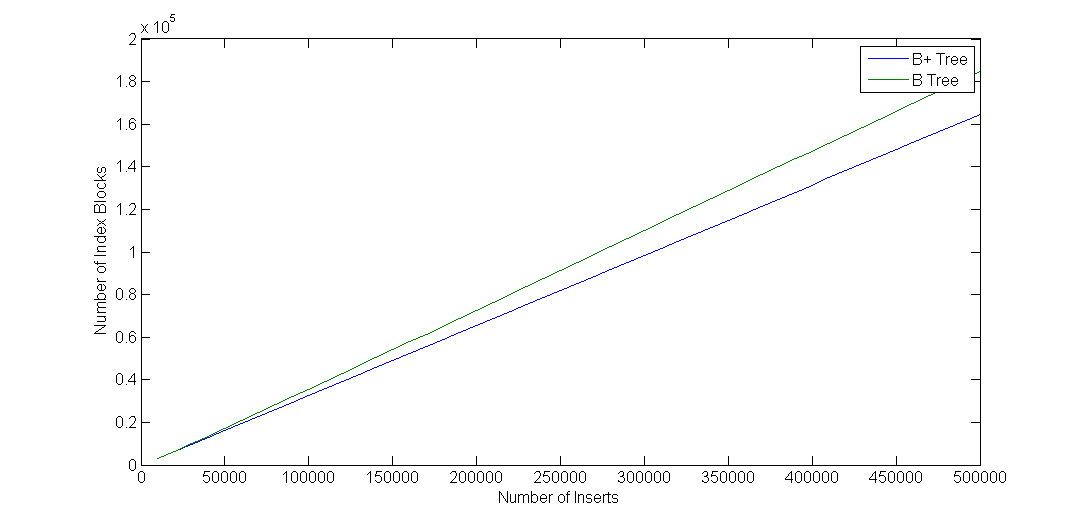
\includegraphics[width=1.2\linewidth]{Images/figure1.png}}
\caption{Index Blocks as a function of inserts for B-tree and B+-tree}
\end{figure}

First, and most obviously, as shown here in Figure 8, a B-tree uses more blocks than a B+-tree as the number of inserts increases.  Both scales here are linear, so we can see that both are a linear function of number of inserts.\\

\begin{figure}[h!]
\centerline{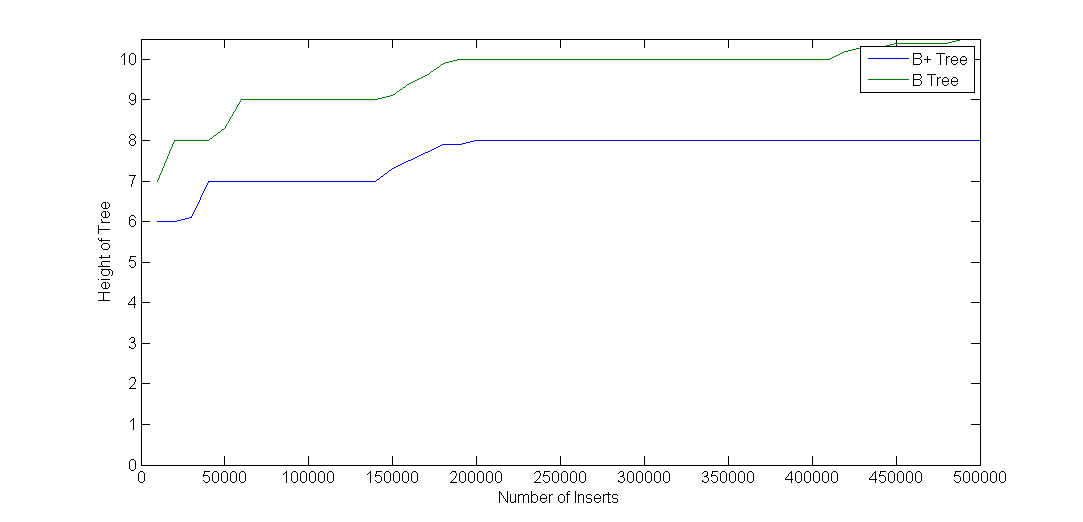
\includegraphics[width=1.2\linewidth]{Images/figure2.png}}
\caption{Height of trees, on average, given number of inserts}
\end{figure}

In Figure 9 we see the height required, on average, for a tree with a given number of inserts.  As above, B+-trees are more space-efficient, maxing out at around 8 nodes in the tree, where B-trees require around 10 for very large numbers of inserts.\\

\begin{figure}[h!]
\centerline{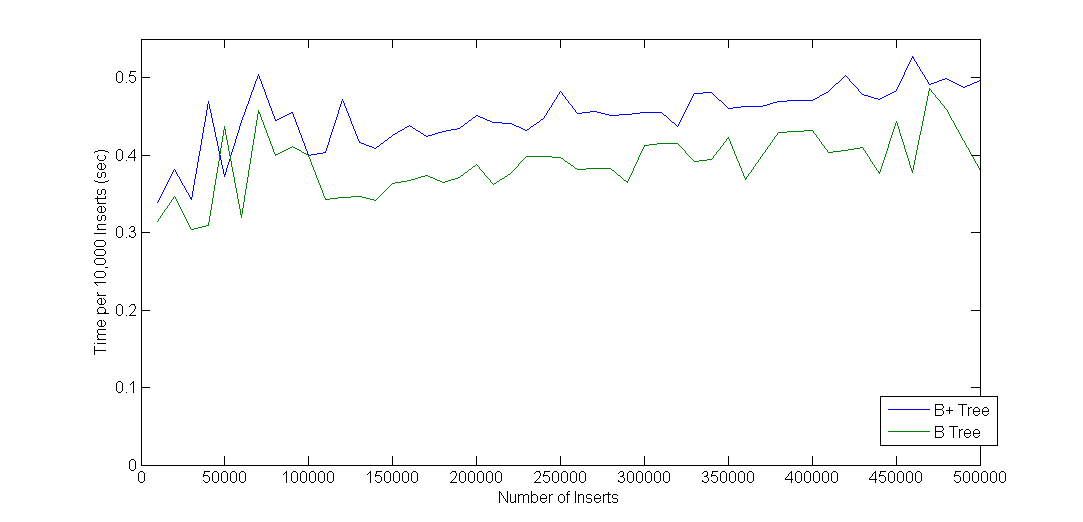
\includegraphics[width=1.2\linewidth]{Images/figure3.png}}
\caption{Time efficiency of the B and B+-trees}
\end{figure}

In figure 10 we can see what we get for our inefficient space usage in the B-tree vs. B+-tree.  The B-tree is consistently faster to use than the B+-tree, requiring around 0.4 s / 10000 inserts instead of 0.5 s / 10000 inserts of the B+-tree.  We should, however, recall that this experiment was done without using swap space on disk, and the disk operations are more costly than the in-memory operations.  That is the purpose of using B+-trees instead of B-trees: to use in-memory space more efficiently and prevent having to swap to disk in the eventual case where the index cannot be held in memory.\\

\begin{figure}[h!]
\centerline{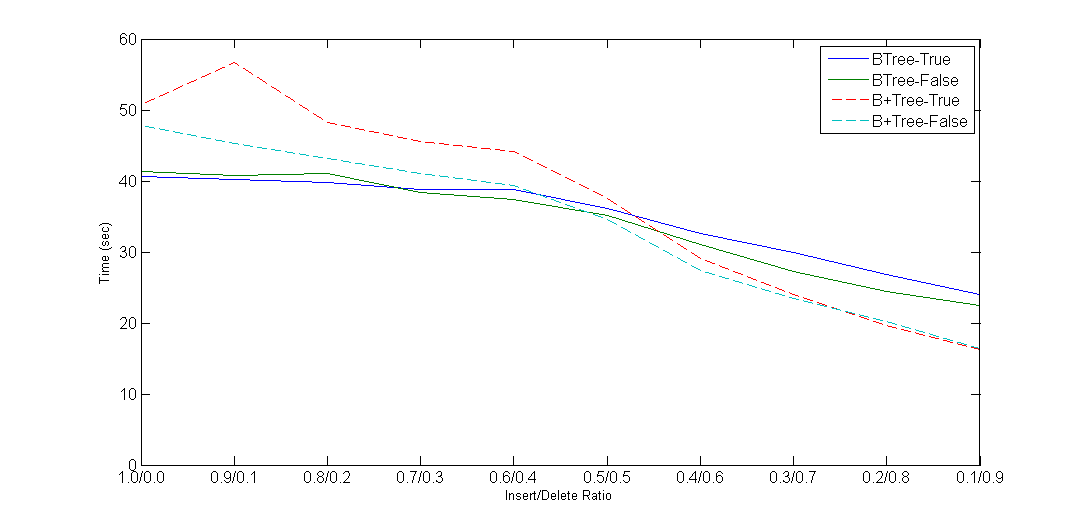
\includegraphics[width=1.2\linewidth]{Images/figure5.png}}
\caption{Comparison of different trees performance using different coalescing settings}
\end{figure}

In figure 11 we have the comparison between different trees using different coalescing settings.  We see that the B+-tree performs better than the B-tree until the insert/delete ratio is high enough, and that the non-coalescing trees follow the coalescing trees in general trend.  For the B-tree, the non-coalescing version performs better under heavy insert load, and for the B+-tree, the non-coalescing tree performs slightly better under delete-heavy load.  This makes sense: the B+-tree with a delete-heavy load will mostly be small nodes, which will cause a lot of underflows that the coalescing version will have to deal with.  The B-tree with the heavy insert-load will need to do slightly more maintenance than the non-coalescing version.  So, we can see here that under very specific circumstances, we can get a very slightly better bit of performance out of a non-coalescing version.  This marginally-better performance will be amplified substantially when we end up swapping to disk, as we would in most DBMSs.\\

\begin{figure}[h!]
\centerline{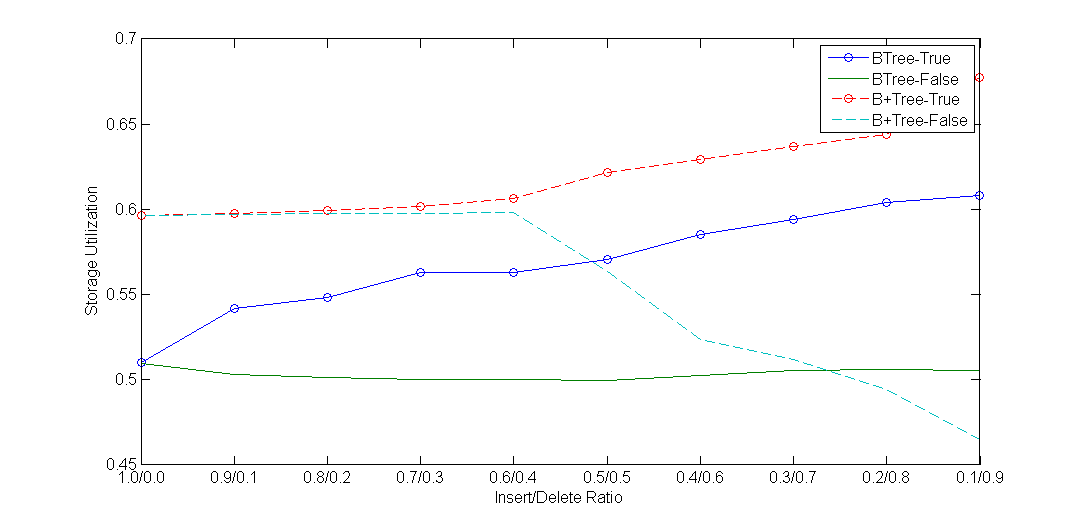
\includegraphics[width=1.2\linewidth]{Images/figure4.png}}
\caption{Comparison of different trees storage utilization using different coalescing settings}
\end{figure}

In figure 12 we see the performance in storage utilization for the different kinds of trees, using different coalescing settings.  As we would expect, the B+-tree makes better use of its storage than the B-tree, and both non-coalescing versions make very poor use of their storage as the insert-delete ratio increases.\\

\clearpage

\section{Conclusion}

We conclude that, under certain very specific circumstances, it might be a good idea to turn off coalescing in a database.  It certainly fails to impact performance substantially to remain uncoalesced for a short period of time, and therefore it makes sense that most enterprise database systems have a specific "COALESCE" command which will cause the database to coalesce its indices.  This command could be called under situations of very low load on the database, and get the best of both worlds: fast response time overall, and better storage utilization.

\end{document}